% !TEX encoding = UTF-8
% !TEX TS-program = pdflatex
% !TEX root = ../tesi.tex

%**************************************************************
\chapter{Analisi e progettazione}
\label{cap:analisi}
%**************************************************************

\intro{Il seguente capitolo descrive l'analisi, la progettazione iniziale, e le soluzioni addottate durante la codifica}\\


%**************************************************************
\section{Analisi e progettazione iniziale}
Le funzionalità da implementare e gli obbiettivi da raggiungere erano già ben definiti all'inizio del progetto, in quanto l'analisi funzionale è stata fornita dal Product owner insieme ad una prima definizione del product backlog.
Per questo motivo la fase di analisi dei requisiti da parte del team di sviluppo è stata molto breve e si è concentrata principalmente su come le funzionalità del prodotto dovessero essere fruibili all'utente finale. La progettazione del software non è avvenuta solamente all'inizio, ma si è protratta durante tutto il periodo di stage. Questo ha garantito maggior flessibilità nell'implementazione delle funzionalità e ha favorito l'utilizzo di Scrum. Tale scelta tuttavia ha anche introdotto il rischio che una debole progettazzione iniziale potesse causare problemi nelle settimane a venire. Questo rischio è stato subito mitigato grazie ad un attenta progettazione della base di dati pensando, nel miglior modo possibile, alle entità, a come esse fossero in relazione tra di loro e alla logica necessaria per implementare le funzionalità richieste. Inoltre, in quanto JHipster utilizza uno stack tecnologico ben definito, e impone dei vincoli architetturali da seguire, tale rischio è ulteriormente ridotto poiché non è necessario progettare l'architettura del prodotto.
Nel corso di questo capitolo vengono descritte le principali attività di progettazione svolte durante il corso dello stage.

%**************************************************************
\section{Progettazione del database}
La progettazione del database è stata una delle attività più importanti e deteneva un alto grado di priorità anche nel Product backlog. La progettazione del database è stata divisa in due parti: la prima mirata a individuare le entità partendo dall'analisi dei requisiti fatta dal Product owner, mentre la seconda mettendo in relazione tali entità aggiungendo tabelle se necessario. Per quanto riguarda la vera e propria implementazione del database è stato sfruttato un tool fornito da JHipster ovvero \href{https://start.jhipster.tech/jdl-studio/}{JDLStudio}, che verrà descritto in modo dettagliato successivamente nel corso di questa sezione.

\subsection{Entità}
Durante la progettazione della base di dati sono state definite le entità descritte di seguito.
Per ciascuna di esse viene riportata una breve descrizione e la lista dei suoi campi dati corredata da tipo di dato, nella lista seguente non vengono riportate chiavi primarie ne chiavi esterne poiché l'inserimento di tali campi dati è automatizzato e verrà descritto dettagliatamente nella sezione relativa alle \hyperref[rel]{relazioni tra entità}.
Mentre si stava effettuando la progettazione del database è sorto il problema di come si volessero salvare i \gls{contenutog} e i template. Si è optato di suddividere i contenuti in pagine, ognuna delle quali può contenere uno o più elementi multimediali e/o testuali. Inoltre in uno stesso contenuto si può selezionare un template diverso per ogni pagina. Per quanto riguarda i template, i quali sono definiti a monte dal team di sviluppo, si è scelto di strutturarli definendo un template al cui interno sono contenuti vari item che possono essere sia testuali che multimediali. Questo rende tutto il più modulare possibile, in quanto non pone limiti né in fase di creazione di un contenuto, né nella definizione dei template e nel loro utilizzo. 
\subsubsection{Content}
Definisce un contenuto informativo, i suoi campi dati sono:
\begin{itemize}
    \item name (String): Nome del contenuto;
    \item state (State): Enumerazione che definisce i possibili stati di un contenuto;
    \item description (String): descrizione del contenuto informativo;
    \item slideTime (Integer): durata delle slide di un contenuto;
\end{itemize}

\subsubsection{ContentPage}
Definisce una pagina inserita in un contenuto. Ogni contenuto può avere più pagine che scorreranno come slide durante la visualizzazione dello stesso; ogni pagina contiene degli item multimediali o testuali. I suoi campi dati sono:
\begin{itemize}
    \item pageNumber (Integer): numero della pagina all’interno di un contenuto.
\end{itemize}

\subsubsection{MultimediaItem}
Definisce un item multimediale (immagine o video) contenuto in una pagina. I suoi campi dati sono:
\begin{itemize}
    \item path (String): percorso del file multimediale caricato sul server, nel caso il caricamento delle immagini avvenga su NAS;
    \item resolution (Resolution): enumerazione che definisce la risoluzione dell'immagine caricata;
    \item multimediaFile (Blob): file multimediale caricato su database, nel caso il caricamento non avvenga su NAS;
\end{itemize}

\subsubsection{TextItem}
Definisce un testo contenuto in una pagina. I suoi campi dati sono:
\begin{itemize}
    \item text (Blob): contenuto testuale inserito in una pagina.
\end{itemize}

\subsubsection{Template}
Definisce un template che verrà utilizzato dalle pagine di un contenuto. Ogni pagina può utilizzare template definiti a monte che determinano come immagini, video e contenuti testuali vengono disposti nella pagina al momento della presentazione. I suoi campi dati sono:
\begin{itemize}
    \item previewImage (Blob): immagine di preview del template, utilizzata per aiutare l'utente a capire come questo è definito;
    \begin{figure}[h]
        \begin{center}
        
\includegraphics[width=0.18\textwidth]{textImage50_50}
        \caption{Immagine di preview di un template contenente un testo e un'immagine}
        \label{fig:figure15}
        \end{center}
    \end{figure}
    \item templateHTML (Blob): contiene l'html del template;
    \item name (String): Nome del template.
\end{itemize}

\subsubsection{TemplateItem}
Definisce un item all'interno di un template. Per item si intende un singolo testo, immagine o video. Questa entità viene utilizzata in fase di creazione e di visualizzazione di un contenuto ed è utilizzata per sapere cosa va inserito in una pagina che utilizza un determinato template. 
I suoi campi dati sono:
\begin{itemize}
    \item description (String): descrizione dell'item del template (e.g. video a schermo intero);
    \item type (itemType): enumerazione che definisce il contenuto che viene inserito in quell’area del template;
    \item TemplateArea (Integer): area del template in cui un certo oggetto va inserito, utilizzato in fase di preview per inserire immagini, video e testi al posto giusto all'interno del template.
\end{itemize}

\subsubsection{CSS}
Definisce il CSS utilizzato da uno o più template. I suoi campi dati sono:
\begin{itemize}
    \item templateCSS (Blob): contiene il CSS utilizzato da uno o più template.
\end{itemize}

\subsubsection{CustomAudit}
Entità definita per implementare il sistema di Audit. I suoi campi dati sono:
\begin{itemize}
    \item action (Action): enumerazione che definisce il tipo di azione registrata negli audit;
    \item description (String): descrizione dettagliata dell'azione effettuata;
    \item timestamp (Instant): data e ora in cui l'azione registrata è stata eseguita.
\end{itemize}

\subsubsection{User}
Entità predefinita in JHipster contenente tutte le informazioni necessarie per registrare un utente. Per utilizzarla è sufficiente definire relazioni ad essa.

\subsection{Enumerazioni}
Durante la progettazione della base di dati, in alcuni casi, si è ritenuto necessario definire alcuni campi dati come enumerazione al posto di utilizzare una semplice stringa di testo.
Questo garantisce maggior controllo e impone vincoli che evitano il verificarsi di errori relativi all'utilizzo di nomi diversi per esprimere lo stesso concetto. Le enumerazioni definite durante la progettazione del database sono le seguenti.

\subsubsection{State}
Lista dei possibili stati di un contenuto informativo, ovvero: \textit{CREATED, TO\textunderscore{}ASSOCIATE, ASSOCIATED, TO\textunderscore{}AUTHORIZE, AUTHORIZED, PUBLISHED}.

\subsubsection{Resolution}
Lista delle possibili risoluzioni di un elemento multimediale, ovvero: \textit{HIGH, MEDIUM, LOW}.

\subsubsection{ItemType}
Lista delle diverse tipologie di template item, ovvero: \textit{IMAGE, VIDEO, TEXT}.

\subsubsection{Action}
Lista delle azioni da registrare nel sistema di auditing che possono essere effettuate da un utente, ovvero: \textit{CREATE, DELETE, UPDATE, AUTHENTICATION\textunderscore{}SUCCESS, AUTHENTICATION\textunderscore{}FAILURE, LOGOUT, TIMEOUT}.

\subsection{Relazioni}
\label{rel}
Di seguito vengono evidenziate le relazioni tra le entità descritte in precedenza e ne viene data una breve descrizione.
\subsubsection{Content-ContentPage}
Ogni Content può avere una o più ContentPage, ogni ContentPage è inserita in un solo contenuto.
\subsubsection{Template-ContentPage}
Ogni Template può essere utilizzato da una o più ContentPage, ogni ContentPage utilizza un solo Template.
\subsubsection{Content-page-MultimediaItem}
Ogni ContentPage può contenere uno o più MultimediaItem, ogni MultimediaItem è contenuto in una sola pagina.
\subsubsection{ContentPage-TextItem}
Ogni ContentPage può contenere uno o più TextItem, ogni TextItem è contenuto in una sola pagina.
\subsubsection{Template-TemplateItem}
Ogni Template ha al suo interno uno o più TemplateItem, ogni TemplateItem fa riferimento a un solo Template.
\subsubsection{MultimediaItem-TemplateItem}
Ogni MultimediaItem può riferirsi ad un solo TemplateItem, ad ogni TemplateItem possono essere riferiti uno o più MultimediaItem.
\subsubsection{TextItem-TemplateItem}
Ogni TextItem può riferirsi ad un solo TemplateItem, ad ogni TemplateItem possono essere riferiti uno o più TextItem.
\subsubsection{Content-User}
Ogni Content è creato da un solo User, ogni User può creare uno o più content.
\subsubsection{CSS-Template}
Ogni Template può avere uno o più CSS, ogni CSS può essere utilizzato da uno o più Template.
\subsubsection{CustomAudit-User}
Ogni Audit si riferisce ad un solo User, ad ogni User possono essere registrati uno o più Audit.


\subsection{Implementazione}
\subsubsection{JDL Studio}
JDL Studio è un tool fornito da JHipster che permette di definire lo schema entità-relazioni di un database tramite un apposito linguaggio di scripting chiamato, appunto, JDL. Una delle funzionalità più utili di JDLStudio è la possibilità di visualizzare il modello ER, che viene automaticamente aggiornato ad ogni modifica.
\newpage
\subsubsection{Definizione di un'entità in JDLStudio}
Un'entità viene definita in JDL specificando il suo nome e i suoi campi dati. Un esempio di definizione di un'entità è il seguente:
\begin{lstlisting}[caption={Definizione entità Content},label={lst:ent}]
entity Content {
  name String unique,
  state State,
  description String,
  slideTime Integer
}
\end{lstlisting}
\subsubsection{Definizione di un'enumerazione in JDLStudio}
Un'enumerazione viene definita in JDL specificandone il nome e i suoi possibili valori dati. Un esempio di definizione di un'entità è il seguente:
\begin{lstlisting}[caption={Definizione enumerazione State},label={lst:ent}]
enum State {
  CREATED,
  TO_ASSOCIATE,
  ASSOCIATED,
  TO_AUTHORIZE,
  AUTHORIZED,
  PUBLISHED
}
\end{lstlisting}
\subsubsection{Definizione di una relazione in JDLStudio}
Per definire una relazione in JDL bisogna innanzitutto specificare il tipo di relazione (uno a uno, uno a molti, molti a molti). Fatto questo è sufficiente specificare l'entità di partenza della relazione e quella di arrivo. Un esempio di definizione di relazioni in JDL è il seguente:
\begin{lstlisting}[caption={Definizione relazioni uno a molti},label={lst:ent}]
relationship OneToMany {
  Content{page} to ContentPage{content},
  Template{page} to ContentPage{template},
  ContentPage{multimediaItem} to MultimediaItem{page},
  TemplateItem{multimediaItem} to MultimediaItem{templateItem},
  Template{templateItem} to TemplateItem{template},
  ContentPage{textItem} to TextItem{page},
  TemplateItem{textItem} to TextItem{templateItem}
}
\end{lstlisting}
\newpage
\subsubsection{Modello ER}
Il modello ER autogenerato presenta imperfezioni nella visualizzazione delle relazioni, nonostante ciò e stato ritenuto sufficiente per gli scopi del progetto.
\begin{figure}[h]
    \begin{center}
    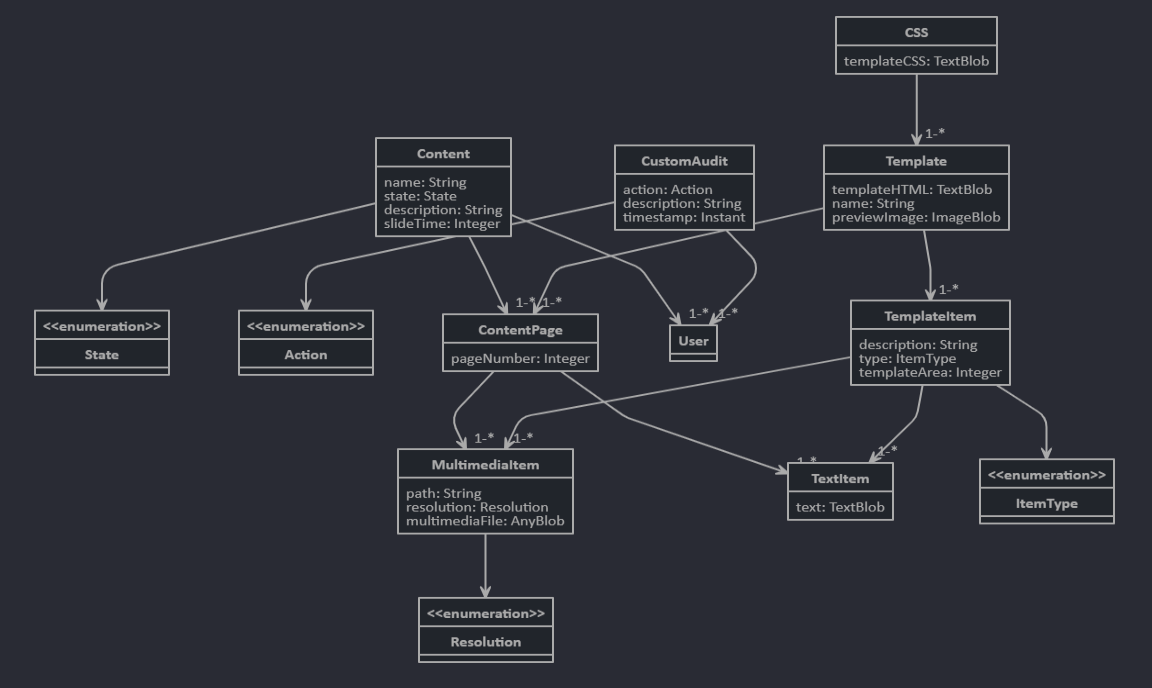
\includegraphics[width=1.2\textwidth]{er}
    \caption{Modello ER generato da JDLStudio}
    \label{fig:figure19}
    \end{center}
\end{figure}

%**************************************************************
\section{Definizione dei template per i contenuti}
In quanto nella progettazione del database è stato scelto di modellare i template in modo che fossero più modulari ed estendibili possibile, è stata necessaria un accurata definizione degli stessi. Si è optato per definire un template di base utilizzato da ogni contenuto informativo, e una serie di template personalizzati utilizzati dalle pagine inserite in un contenuto.
\subsection{Template di base}
Il template di base definito contiene poche informazioni. Definisce infatti la struttura base della pagina html e la funzione per visualizzare le slide. Contiene inoltre vari placeholder utilizzati per inserire dinamicamente le informazioni di un determinato contenuto informativo.
I placeholder definiti sono: 

%**************************************************************
\section{Definizione dei servizi di backend}

